\documentclass[12pt]{report}
\usepackage{amsmath}
\usepackage{ragged2e}
\usepackage{graphicx}
\graphicspath{ {./img/} }
\setlength\parindent{0pt}

\newcommand{\thn}{\textsuperscript{th}}

\newcommand{\twopartdef}[4]
{
	\left\{
	\begin{array}{ll}
		#1 & \mbox{} #2 \\
		#3 & \mbox{} #4
	\end{array}
	\right.
}

\newcommand{\threepartdef}[6]
{
	\left\{
	\begin{array}{lll}
		#1 & \mbox{} #2 \\
		#3 & \mbox{} #4 \\
		#5 & \mbox{} #6
	\end{array}
	\right.
}

\begin{document}

\Large
\centering
AMS310 Homework 3

\justify
\normalsize

Kuba Gasiorowski\\
ID: 109776237\\

\noindent \textbf{1a.} In order to prove $f(x)$ is a pdf we must show the following:
\begin{enumerate}
	\item $\forall x, f(x) \geq 0$
	\item $\int_{-\infty}^{\infty} f(x)dx = 1$
\end{enumerate}

\noindent (1) is obvious, since it is given that $ f(x) = \frac{1}{3}, 0 < x < 3 $, and we can assume $f(x) = 0, x \leq 0 \;\text{and}\; x \geq 3$. Thus $\forall x, f(x) \geq 0$.\\

\noindent (2) can be found by taking the following integral: 
\begin{align*}
\int_{0}^{3}\frac{1}{3}dx &= 1\\
\frac{1}{3}\int_{0}^{3}1dx &= 1\\
\frac{1}{3}\left[x\right]_0^3 &= 1\\
\frac{1}{3}(3 - 0) &= 1\\
1 &= 1
\end{align*}

\noindent Thus $f(x)$ is a pdf. \\

\pagebreak

\noindent \textbf{b.} To find the mean ($\mu$) of $f(x)$:

\begin{align*}
\mu &= \int_{-\infty}^{\infty} xf(x)dx \\
\mu &= \int_0^3 x\frac{1}{3}dx \\
\mu &= \frac{1}{3}\int_0^3 xdx \\
\mu &= \frac{1}{3} \cdot \left[\frac{x^2}{2}\right]_0^3 \\
\mu &= \frac{1}{3} \cdot \left(\frac{3^2}{2} - \frac{0^2}{2}\right)\\
\mu &= \boxed{\frac{9}{6} = 1.5}
\end{align*}

\noindent And then the variance ($\sigma$):

\begin{align*}
\sigma^2 &= \int_{-\infty}^{\infty} x^2f(x)dx - \mu^2\\
\sigma^2 &= \int_{0}^{3} \frac{1}{3}x^2dx - 2.25\\
\sigma^2 &= \frac{1}{3}\int_{0}^{3}x^2dx - 2.25\\
\sigma^2 &= \frac{1}{3} \cdot \left[ \frac{x^3}{3} \right]_0^3 - 2.25\\
\sigma^2 &= \frac{1}{3} \cdot 9 - 2.25\\
\sigma^2 &= 0.75\\
\sigma &= \boxed{\sqrt{0.75} \approx 0.866}\\ 
\end{align*}

\pagebreak

\noindent \textbf{e.} Find $P(\frac{1}{2} < X < \frac{5}{2})$:
\begin{align*}
(\frac{1}{2} < X < \frac{5}{2}) &= \int_{\frac{1}{2}}^{\frac{5}{2}}\frac{1}{3}dx\\
&= \frac{1}{3}\int_{\frac{1}{2}}^{\frac{5}{2}}1dx\\
&= \frac{1}{3}\left[x\right]_{\frac{1}{2}}^{\frac{5}{2}}\\
&= \frac{1}{3}\left(\frac{5}{2} - \frac{1}{2}\right)\\
&= \boxed{\frac{2}{3} \approx .66\overline{6}}\\
\end{align*}

\noindent \textbf{f.} Find $P(X > 1)$:
\begin{align*}
P(X > 1) &= \int_1^{\infty}f(x)dx\\
&= \int_{1}^{3}\frac{1}{3}dx\\
&= \frac{1}{3}\int_{1}^{3}1dx\\
&= \frac{1}{3}\left[x\right]_1^3\\
&= \frac{1}{3}(3-1)\\
&= \boxed{\frac{2}{3} \approx .66\overline{6}}
\end{align*}

\pagebreak

\noindent \textbf{g.} Find the 40\thn percentile.

\begin{align*}
\int_{0}^{x_{0.4}}f(x)dx &= 0.4\\
\int_{0}^{x_{0.4}}\frac{1}{3}dx &= 0.4\\
\frac{1}{3}\int_{0}^{x_{0.4}}1dx &= 0.4\\
\frac{1}{3}[x]_0^{x_{0.4}} &= 0.4\\
\frac{1}{3}x_{0.4} &= 0.4\\
x_{0.4} &= \boxed{1.2}
\end{align*}

\noindent \textbf{2a.} Given $N(90, 225)$, find $P(X > 80)$.\\\\
\noindent We have $\mu = 90$, $\sigma^2=225 \Rightarrow \sigma = 15$, and $x = 80$.
\begin{align*}
z &= \frac{x - \mu}{\sigma}\\
z &= \frac{80 - 90}{15}\\
z &= -.66
\end{align*}

\noindent Then using the normal tables, we get $.2546$ as the area underneath the curve to the left of $z = -0.66$. Since we want to know the area to the right, we subtract that from 1 and get $\boxed{0.7454} = 75.54\%$ as the answer.\\

\noindent \textbf{b.} We use the above formula, except solving for x for the z-score that corresponds to 75\%. The closest z-score to .75 is 0.68. Then we have:
\begin{align*}
\frac{x-\mu}{\sigma} &= z\\
x &= z\sigma + \mu\\
x &= 0.68 \cdot 15 + 90\\
x &= 100.2
\end{align*}

\noindent Thus the weight that separates the top 25\% of the male sheep is approximately \boxed{100.2 \text{ pounds}}.\\

\noindent \textbf{3a.} We have $N(\mu = 115000, \sigma^2 = 10000^2)$. Find $P(X > 130000)$. \\
\begin{align*}
z &= \frac{x - \mu}{\sigma}\\
z &= \frac{130000 - 115000}{10000}\\
z &= 1.5
\end{align*}

\noindent Then using the normal tables to convert the z-score to a percent, we obtain 0.9332. Then we find 1 - 0.9332 and get 0.0668 or \boxed{6.68\%} of timing belts last 130k miles or more.\\

\noindent \textbf{b.} Find $P(X < 100000)$.

\begin{align*}
z &= \frac{x-\mu}{\sigma}\\
z &= \frac{100000 - 115000}{10000}\\
z &= -1.5
\end{align*}

\noindent Using the normal tables: $z = -1.5 \Rightarrow 0.0668$. Thus the chance of a timing belt failing at less than 100k is about 6.68\%.\\

\noindent \textbf{c.} First we find the z-score that corresponds to .75, which is $\approx 0.68$. Then we plug and chug.
\begin{align*}
x &= z\sigma + \mu\\
x &= 0.86 \cdot 10000 + 115000\\
x &= \boxed{121800 \text{ miles}}
\end{align*}

\noindent \textbf{4.} First, we have $\lambda = 30$ and $P(X) \Rightarrow F(x) = 1- e^{-\frac{x}{\lambda}}$
\begin{align*}
P(X < 25) &= 1-e^{-\frac{25}{30}}\\
&= 1-e^{-\frac{5}{6}}\\
&\approx 1-0.4346\\
&\boxed{\approx 0.5654}
\end{align*}

\begin{align*}
P(X > 35) &= 1 - P(X < 35)\\
&= 1 - \left(1 - e^{-\frac{35}{30}}\right)\\
&= e^{-\frac{6}{5}}\\
&\approx \boxed{0.3012 \approx 30.12\%}
\end{align*}

\begin{align*}
P(25 < X < 35) &= P(X < 35) - P(X < 25)\\
&= (1-P(X > 35)) - P(X < 25)\\
&= (1 - 0.3012)-0.5654\\
&= \boxed{0.1334 = 13.34\%}
\end{align*}

\noindent \textbf{b.}
\begin{align*}
F(x) &= \frac{1}{2}, \; (\lambda = 30)\\
1-e^{-\frac{x}{30}} &= \frac{1}{2}\\
e^{-\frac{x}{30}} &= \frac{1}{2} \\
-\frac{x}{30} &= \ln{\frac{1}{2}}\\
x &= -30\ln{\frac{1}{2}}\\
x &\approx \boxed{20.79}
\end{align*}

\pagebreak

\noindent \textbf{5a.} Since we must satisfy \\

$$ \int_{-\infty}^{\infty} f(x)dx = 1 \Rightarrow \int_{40}^{100}f(x)dx = 1$$\\
\noindent It's easy to see that $f(x) = \frac{1}{60}$ satisfies the above. So we can draw the pdf as follows:\\

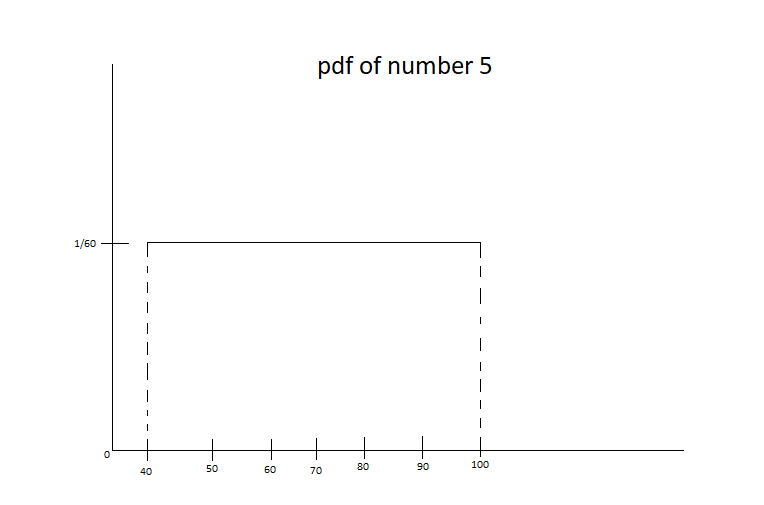
\includegraphics[scale=.7]{hw3_5}

\noindent So in summary, we have:\\

\centering
$f(x) = \twopartdef{\frac{1}{60}}{40 \leq x \leq 100}{0}{\text{otherwise}}$\\
\bigskip
\noindent And\\
\bigskip
$F(x) = \threepartdef{0}{x < 40}{\frac{x}{60}}{40 \leq x \leq 100}{1}{x > 100}$\\

\justify

\pagebreak
\noindent Now we can easily calculate $P(50 < X < 70)$:
\begin{align*}
P(50 < X < 70) &= P(70) - P(50)\\
&= F(70) - F(50)\\
&= \frac{70}{60} - \frac{50}{60}\\
&= \boxed{\frac{1}{3} \approx 33.3\overline{3}\%}
\end{align*}

\noindent And it can be visualized like so:

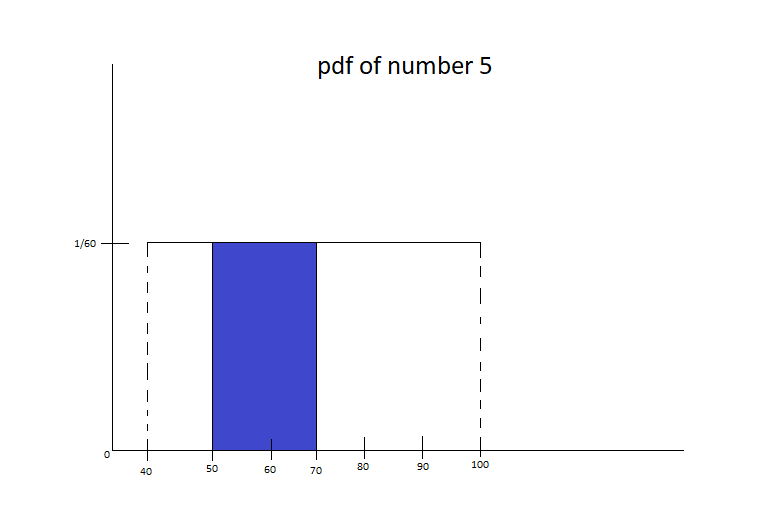
\includegraphics[scale = .7]{hw3_5a}

\pagebreak

\noindent \textbf{b.}

\begin{align*}
P(X < 75) &= F(75) - F(40)\\
&= \frac{75}{60} - \frac{40}{60}\\
&= \boxed{\frac{35}{60} = \frac{7}{12} \approx .5833\overline{3}}
\end{align*}

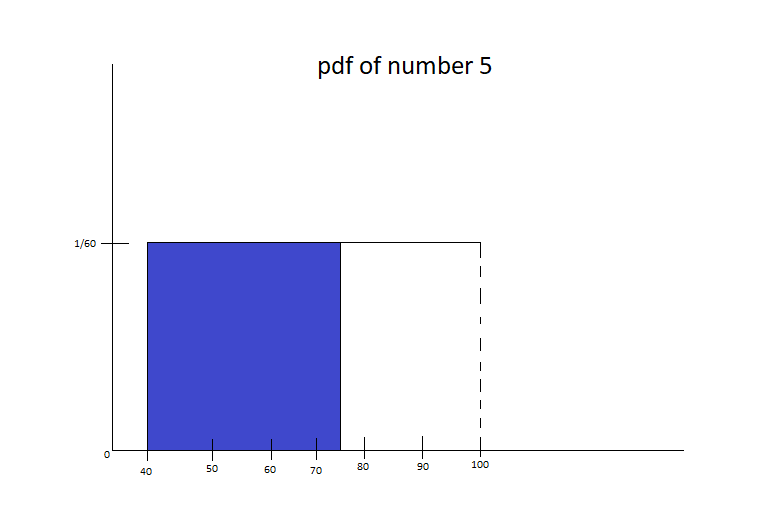
\includegraphics[scale = .7]{hw3_5b}\\

\pagebreak
\noindent \textbf{c.} 
\begin{align*}
P(X > 90) &= P(100) - P(90)\\
&= F(100) - F(90)\\
&= \frac{100}{60} - \frac{90}{60}\\
&= \frac{10}{60} \\
&= \boxed{\frac{1}{6} \approx 0.166\overline{6}}
\end{align*}

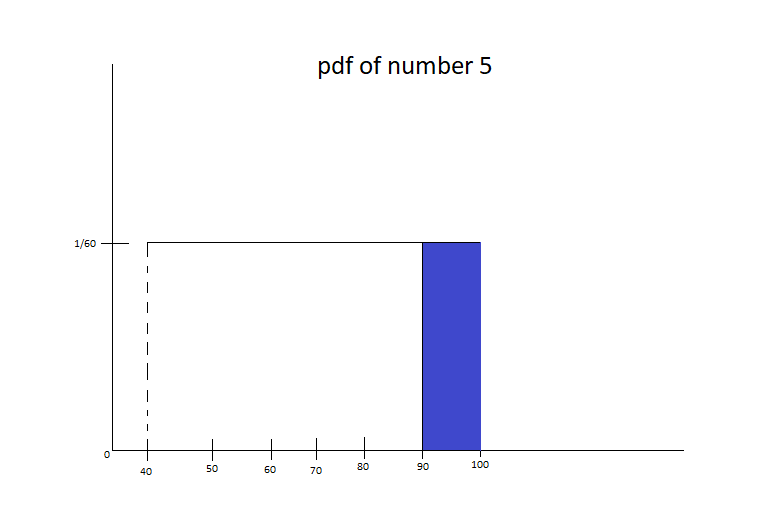
\includegraphics[scale = .7]{hw3_5c}

\pagebreak
\noindent \textbf{d.} 
\begin{align*}
P(x) - P(40) &= 0.95\\
F(x) - F(40) &= 0.95\\
\frac{x-40}{60} &= 0.95\\
x &= \boxed{97}
\end{align*}

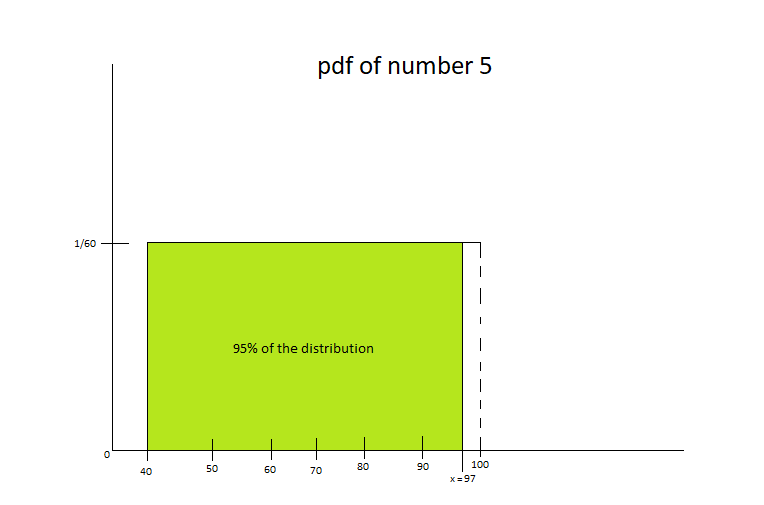
\includegraphics[scale = 0.7]{hw3_5d}\\

\noindent \textbf{6a.} 
\begin{verbatim}
> pexp(.65, 1/.75)
[1] 0.5796496
\end{verbatim}

\noindent \textbf{b.}
\begin{verbatim}
> lambda <- .75
> pexp(2, 1/lambda)-pexp(.75, 1/lambda)
[1] 0.298396
\end{verbatim}

\pagebreak
\noindent \textbf{c.} 
\begin{verbatim}
> qexp(.95, 1/lambda)
[1] 2.246799
\end{verbatim}

\noindent \textbf{7a.} $\mu = E(X) = \alpha\beta = (3)(5) = \boxed{15}$\\
\noindent \textbf{b.} $\sigma^2 = \alpha\beta^2 \Rightarrow \sigma = \sqrt{\alpha\beta^2} = \sqrt{(3)(5)^2} = 5\sqrt{3} \approx \boxed{8.660}$\\
\noindent \textbf{c.} 
\begin{verbatim}
> pgamma(4.5, 3, 1/5)
[1] 0.06285693
\end{verbatim}

\noindent \textbf{d.}
\begin{verbatim}
> pgamma(5, 3, 1/5)-pgamma(2, 3, 1/5)
[1] 0.07237507
\end{verbatim}

\noindent \textbf{8a.} The pdf will look like this:\\ 
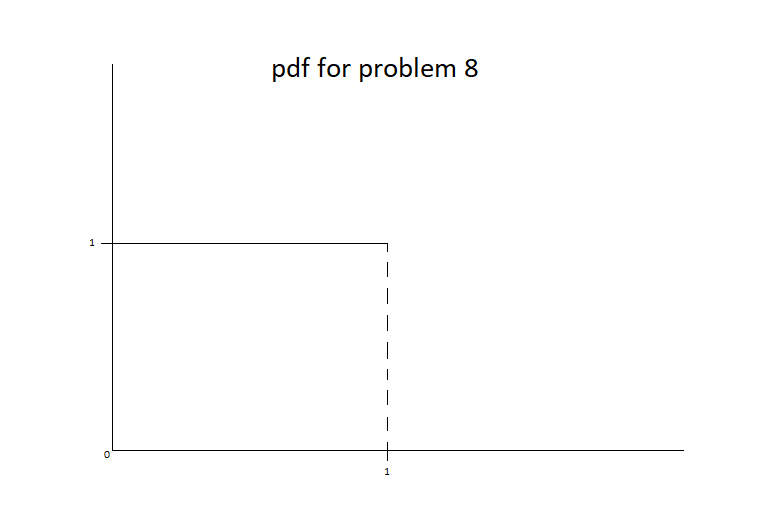
\includegraphics[scale = .7]{hw3_8}

\noindent \textbf{b.} This is also known as a uniform(0,1) distribution.

\noindent \textbf{c.} The cdf is just the area function of the pdf. So it'll look like the following:\\
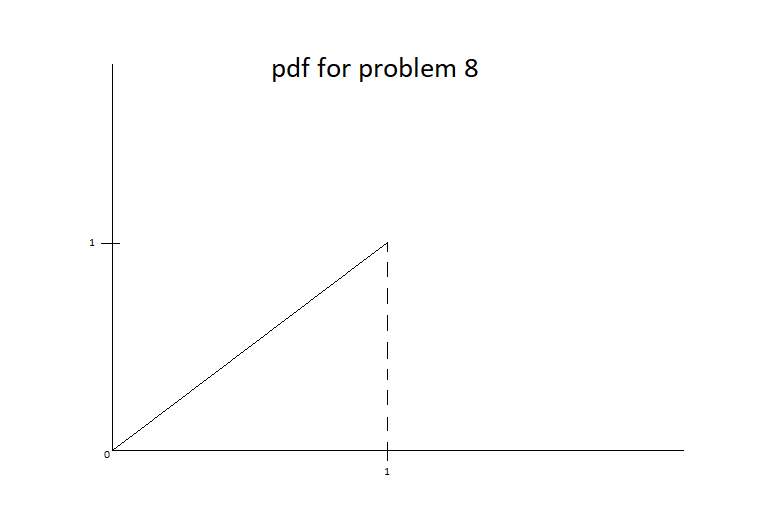
\includegraphics[scale = .7]{hw3_8c}

\noindent \textbf{9a.} $\mu = np = 1000(0.15) = 150$\\
$\sigma = \sqrt{np(1-p)} = \sqrt{1000(0.15)(0.85)} \approx11.291$\\

\begin{align*}
P(X < 125) &= P\left(Z \leq \frac{(X-0.5) - \mu}{\sigma}\right)\\
&= P\left(Z \leq \frac{124.5 - 150}{11.291}\right)\\
&= P(Z \leq -2.25)\\
&= \boxed{.0122}
\end{align*}

\noindent \textbf{b.} 
\begin{align*}
P(X \geq 150) &= P\left(Z \geq \frac{(X - 0.5)-\mu}{\sigma}\right)\\
&= P\left(Z \geq \frac{150.5 - 150}{11.291}\right)\\
&= P(Z \geq 0.0442)\\
&= 1 - 0.5160 = \boxed{0.4840}
\end{align*}

\noindent \textbf{c.} 
\begin{verbatim}
> pbinom(125, 1000, 0.15)
[1] 0.01349891
> 1 - pbinom(150, 1000, 0.15)
[1] 0.4782311
\end{verbatim}

\noindent \textbf{10a.}

\end{document}
